\begin{frame}{Finding the Best Model}

% run on a single machine
Tested Classifiers

\begin{itemize}
\item Naive Bayes 
\item Logistic Regression
\item Neural Network
\item Support Vector Machine
\item Adaboost
\item Hoeffding tree
\item Decision Stump
\end{itemize}
%\vspace{20cm}
Data \begin{itemize}
		\item 2/3 Training
		\item 1/3 Testing
     \end{itemize}
\end{frame}

\begin{frame}{Finding the Best Model}

\begin{figure}[!htb]
\centering
  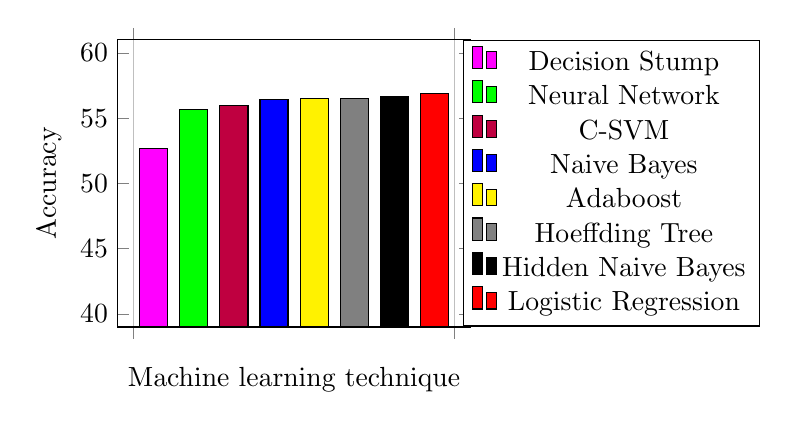
\begin{tikzpicture}
    \begin{axis}[
      %x tick label style={/pgf/number format/1000 sep=},
      xticklabel=\empty,
      ylabel=Accuracy,
      xlabel=Machine learning technique,
      enlargelimits=0.05,
      legend style={at={(1.4,1.0)},
        anchor=north,legend columns=1},
      ybar interval=0.7,
      width=.50\textwidth,
      ymin=40, ymax=60,
      reverse legend,
      ]
      \addplot[fill=red] coordinates {(1,56.916) 
        (0,2)
      };
      \addplot[fill=black] coordinates {(1,56.6807) 
        (0,56.6807)
      };

\addplot[fill=gray] coordinates {(1,56.48)
        (0,0)
      };      
            
      \addplot[fill=yellow] coordinates {(1,56.479) 
        (0,2)
      };
      \addplot[fill=blue] coordinates {(1,56.4454) 
        (0,56.4454)
      };
      \addplot[fill=purple] coordinates {(1,55.98)
        (0,0)
      };
      \addplot[fill=green] coordinates {(1,55.6555) 
        (0,0)
      };      
      \addplot[fill=Fuchsia] coordinates {(1,52.64)
        (0,0)
      };
      \legend{Logistic Regression,Hidden Naive Bayes,Hoeffding Tree,Adaboost,Naive Bayes,C-SVM,Neural Network, Decision Stump}
    \end{axis} 
  \end{tikzpicture}
%  \caption{ue}\label{fig:besttech}
\end{figure}

\end{frame}

\begin{frame}{Logistic Regression}

\[ L_D(\textbf{w}) = \sum_{n=1}^N (y_n-\hat{y}_n)^2 = \sum_{n=1}^N \left(y_n - \sum_{i=0}^M w_i \phi_i(x_n)\right)^{2} \] 

\end{frame}

\begin{frame}{Logistic Regression}

\[ \hat{y} = \sigma(h_w(x)) = \frac{1}{1+e^{-h_w(x)}} \]

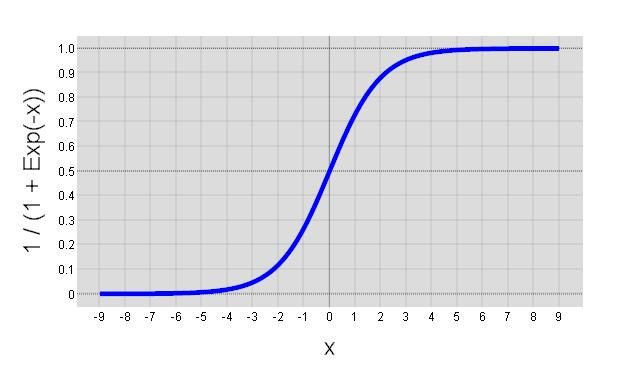
\includegraphics[scale=0.5]{prediction/sigmoid}

\end{frame}	


\begin{frame}{Logistic Regression}


\[E_w(y,h_w(x)) = \begin{cases}
	-ln(\sigma(h_w(x))) &\text{if y = 1}\\	
	-ln(1-\sigma(h_w(x))) &\text{if y = 0}
\end{cases}\]
%
%\includegraphics[scale=0.5]{prediction/-ln(x).png} \\
%\vspace{20cm}
%\includegraphics[scale=0.5]{prediction/-ln(1-x).png}

\begin{figure}
   \includegraphics[width=0.275\textwidth]{prediction/-ln(x).png}
   \hfill
   \includegraphics[width=0.275\textwidth]{prediction/-ln(1-x).png}
\end{figure}

\end{frame}

\begin{frame}{Regularisation}

\[ L(\mathbf{w})
  = L_D(\mathbf{w}) + L_w 
  = \sum_{n=1}^N E_w(y_n, h_w(x_n)) + \frac{\lambda}{2} \sum_{m=1}^{M} {w_m}^2 \] 

\end{frame}

\begin{frame}{Stochastic Gradient Descent}

\[ w_j^{(i)} = w_j^{(i-1)} - \eta \frac{\partial E_{w^{(i-1)}}(y_n, h_{w^{(i-1)}}(x_n))}{\partial w_j^{(i-1)}} \]

\end{frame}


\begin{frame}{Simulated Annealing}

$$\eta_i = \frac{1}{(1+i)^\alpha}$$


With an $\alpha$ chosen in the interval $(0.5,1]$. 

\end{frame}


